\documentclass{beamer}
\usepackage[english]{babel}
\usetheme{CambridgeUS}

\usepackage{caption}
\captionsetup{tableposition=top,figureposition=bottom,font=small}
\usepackage{graphicx}
\usepackage{subfig}
\usepackage{grffile}
\usepackage{booktabs}
\usepackage[absolute,overlay]{textpos}
\usepackage[noend,noline,tworuled]{algorithm2e}
\usepackage{minted}
\setlength{\parskip}{\smallskipamount}

\setbeamertemplate{navigation symbols}{}

\title[]{Screen Space Ambient Occlusion \\\small A WebGL-three.js implementation}

\newsavebox{\authbox}
\sbox{\authbox}{
    \centering
    \begin{minipage}{0.45\linewidth}
        \centering\normalsize
        Ivan Prosperi
    \end{minipage}
}


\author[Ivan Prosperi]{
    \usebox{\authbox}}
\institute[]{Universit\`a degli Studi di Firenze}
\date{}
\logo{\textcolor{black}{
\includegraphics[width=0.10\textwidth]{images/logo_unifi/stemma_grigio.pdf}}}


\AtBeginSection{%
    \begin{frame}
    \tableofcontents[currentsection,subsectionstyle=show/show/hide]
\end{frame}
}

\let\nvec\vec
\def\vec#1{\nvec{\vphantom t\smash{#1}}}


\begin{document}
\definecolor{bg}{rgb}{0.95,0.95,0.95}

\begin{frame}
    \titlepage
    \centering
    Computer Graphics \& 3D Project Report
\end{frame}

\begin{frame}
    \frametitle{Table of contents}
    \tableofcontents[subsubsectionstyle=hide]
\end{frame}

% ##################### START #####################
\section{Introduction}

\subsection{Ambient Occlusion}

\begin{frame}
\frametitle{Ambient Occlusion}
% cosa è, immagini con/senza ao
Ambient occlusion is a shading technique computes the degree of exposure to ambient light in a 3D scene:
\begin{itemize}
    \item open surfaces, planar geometries, ``floating'' geometries: fully exposed to ambient light
    \item corners, hidden geometries, tight gaps between objects, creases: appear shaded in real life, ambient light does not reach them at full intensity
\end{itemize}

\end{frame}

\begin{frame}
\frametitle{Ambient Occlusion Effects}
\begin{figure}
    \centering
    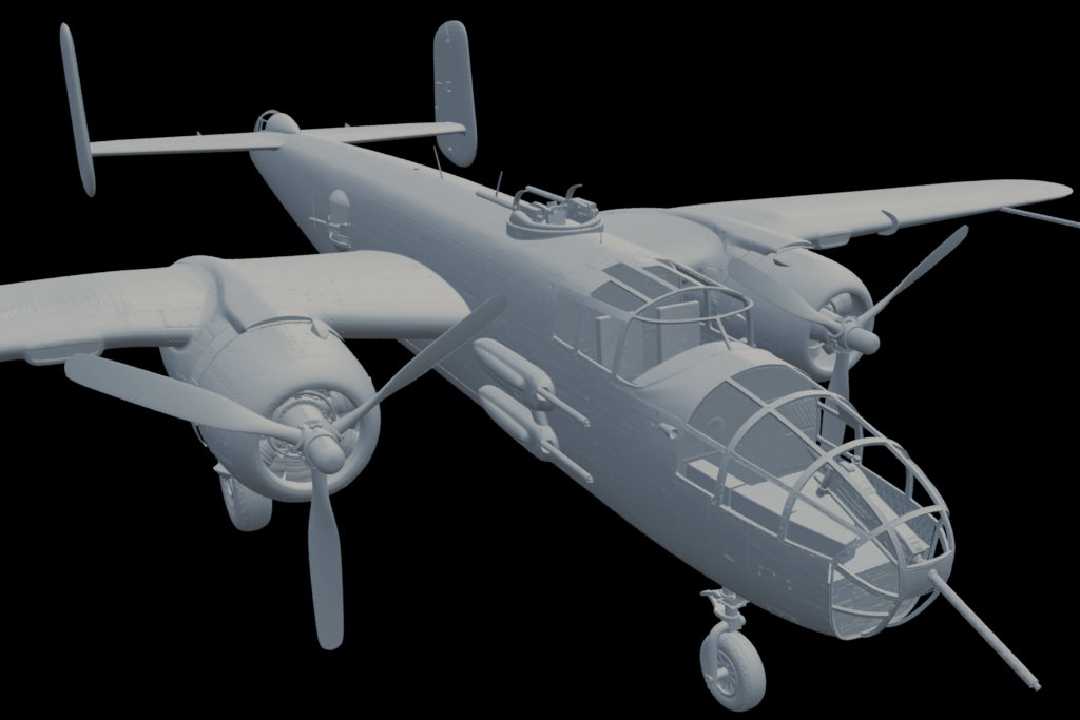
\includegraphics[width=0.8\linewidth]{images/B-25_raw.png}
    \caption{3D object with raw material.\footnotemark}
\end{figure}

\vspace*{-8px}
\footnotetext[1]{\tiny Landis, H. Production-Ready Global Illumination (2004).}
\end{frame}

\begin{frame}
\frametitle{Ambient Occlusion Effects}
\begin{figure}
    \centering
    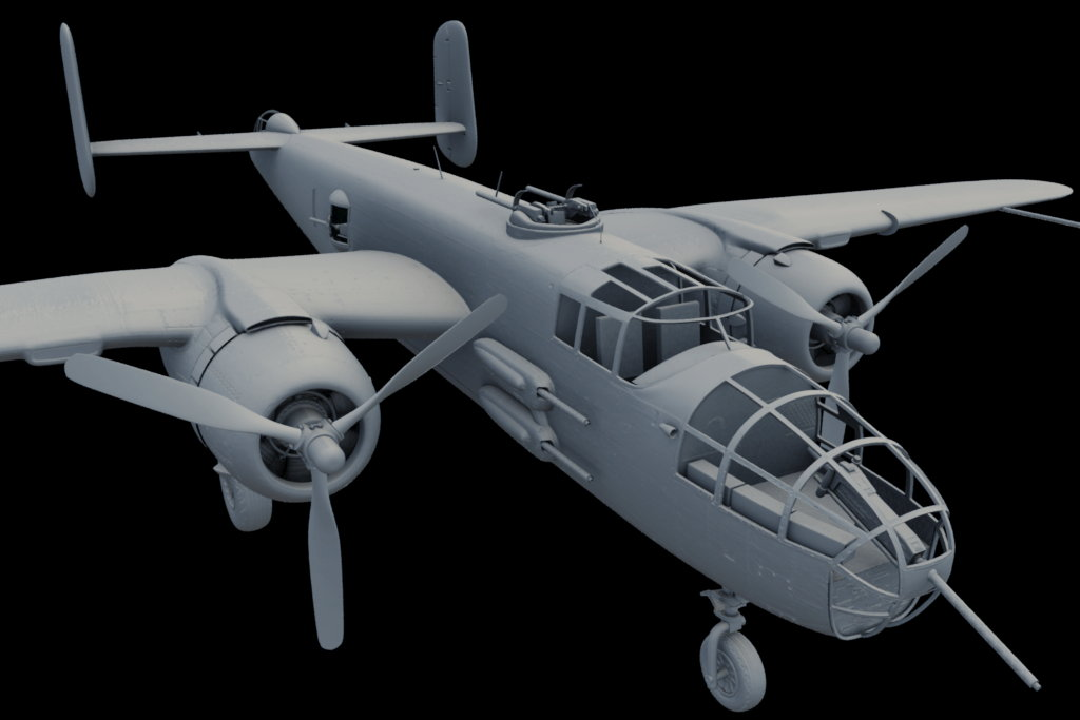
\includegraphics[width=0.8\linewidth]{images/B-25_ao.png}
    \caption{The same object with ambient occlusion applied.}
\end{figure}

\end{frame}

\subsection{Global Illumination}
\begin{frame}[allowframebreaks]
\frametitle{Global Illumination}
% cosa è, immagini indirect light + AO vera + citazione paper AO
% Dire che ao vera è fatta con indirect lighting di GI ma troppo
% costoso in caso di real time
\textbf{Global Illumination (GI)}:
\begin{itemize}
    \item \emph{considers} physically correct light phenomena
    \item \emph{is} a \underline{global method}: illumination at each point is a function of other geometry in the scene
    \item \emph{accounts} for light rays (possibly infinite) bounces
    \item \emph{implements} indirect illumination
    \item \emph{comprises} reflection, refraction, shadows, diffuse inter-reflections, caustics, etc
\end{itemize}

Ambient occlusion approximates some aspects of Global Illumination.

%\end{frame}
\framebreak
%\begin{frame}
%\frametitle{Global Illumination II}
\begin{figure}
    \centering
    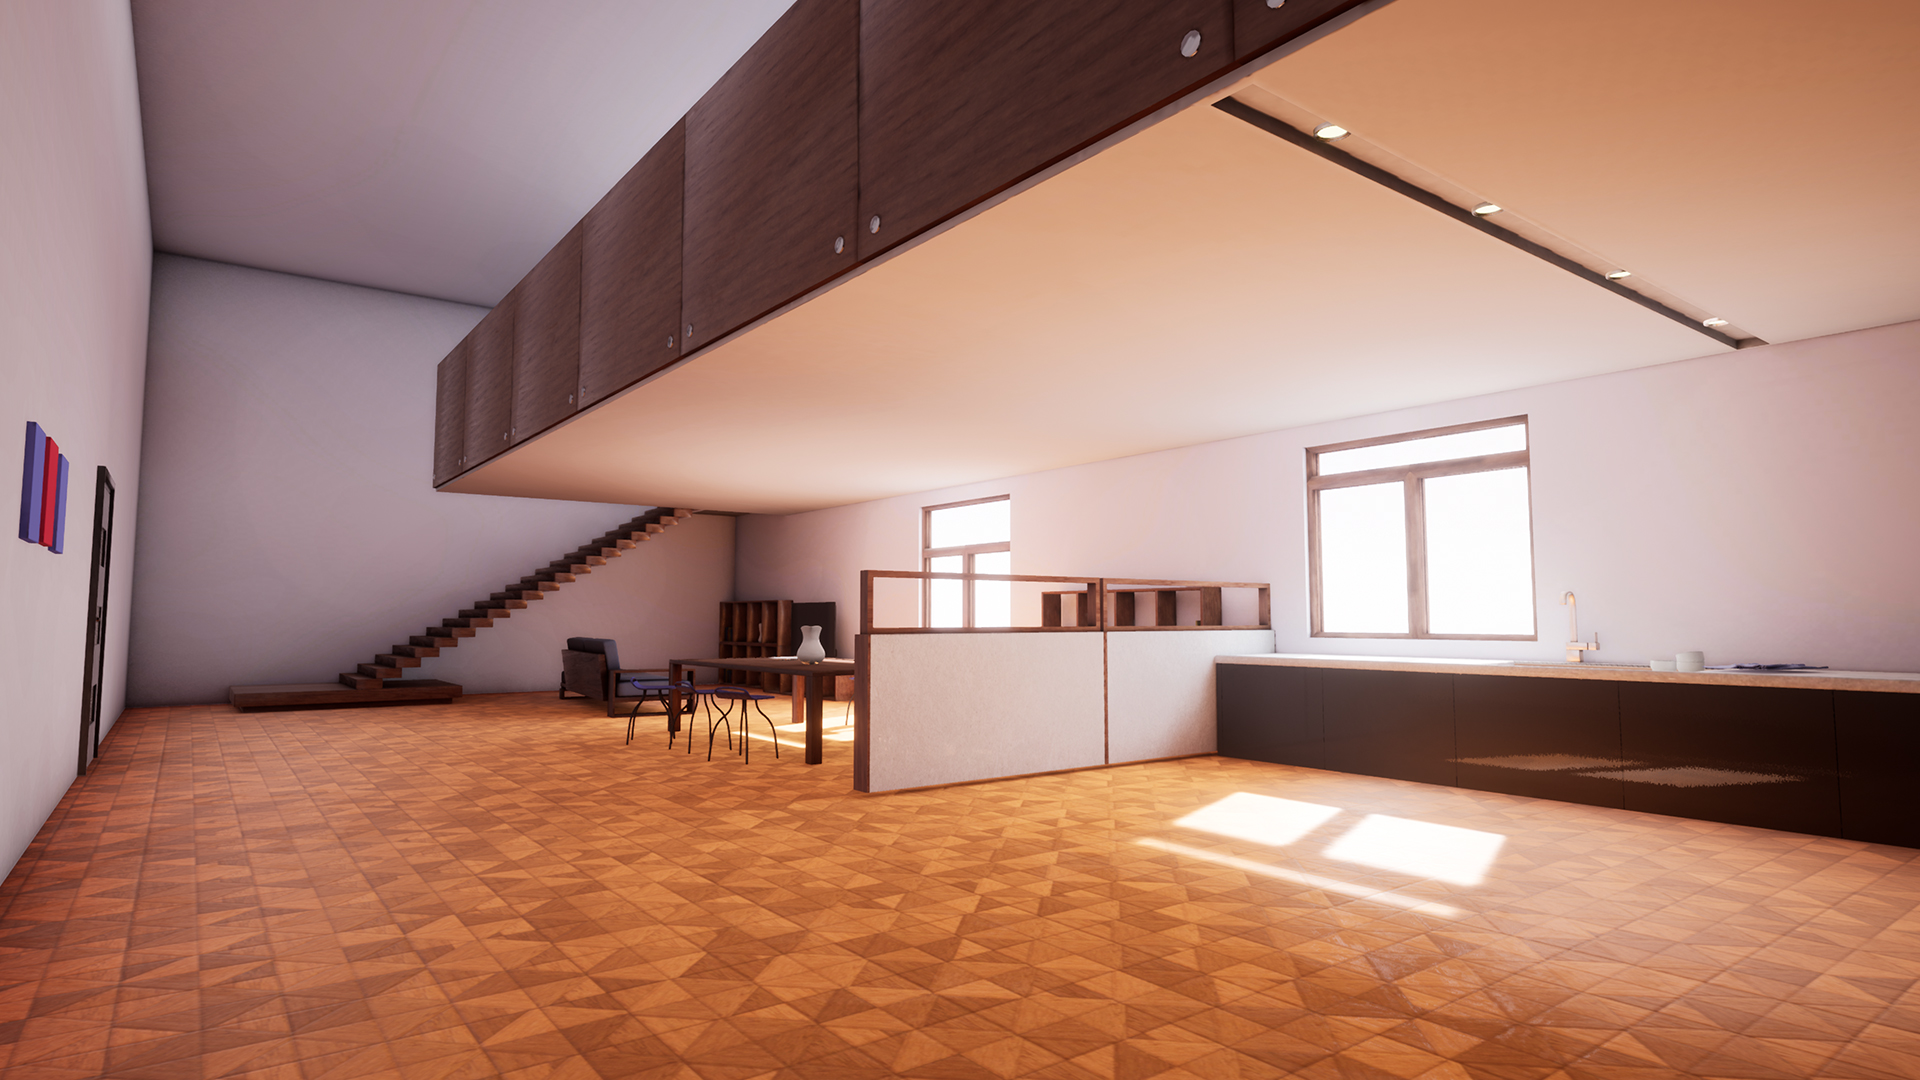
\includegraphics[width=0.9\linewidth]{images/gi_room.jpg}
\end{figure}
%\end{frame}
\framebreak
%\begin{frame}
%\frametitle{Global Illumination III}
Global illumination limits:
\begin{itemize}
    \item a pixel color value depends on the entire scene
    \item light calculation involves solving complex equations
    \item no algorithm exists to implement GI as a whole
\end{itemize}

Furthermore, current real-time graphics hardware is mostly based on rasterization $ \Rightarrow $ ideal for direct illumination computation.

Therefore, \textbf{GI is not reproducible in real time rendering} with the current technologies and hardware.
\end{frame}

\begin{frame}[allowframebreaks]
\frametitle{Multipass Rendering}
% Far vedere esempio di multipass rendering
% Scrivere tipo "used for shadow mapping, normal mapping, etc"
Multipass rendering (and deferred shading) are employed as low-cost approximations for GI effects:
\begin{itemize}
    \item shadow mapping
    \item soft shadows
    \item reflection mapping
    \item light mapping
    \item \textbf{ambient occlusion}
\end{itemize}

\begin{figure}
    \centering
    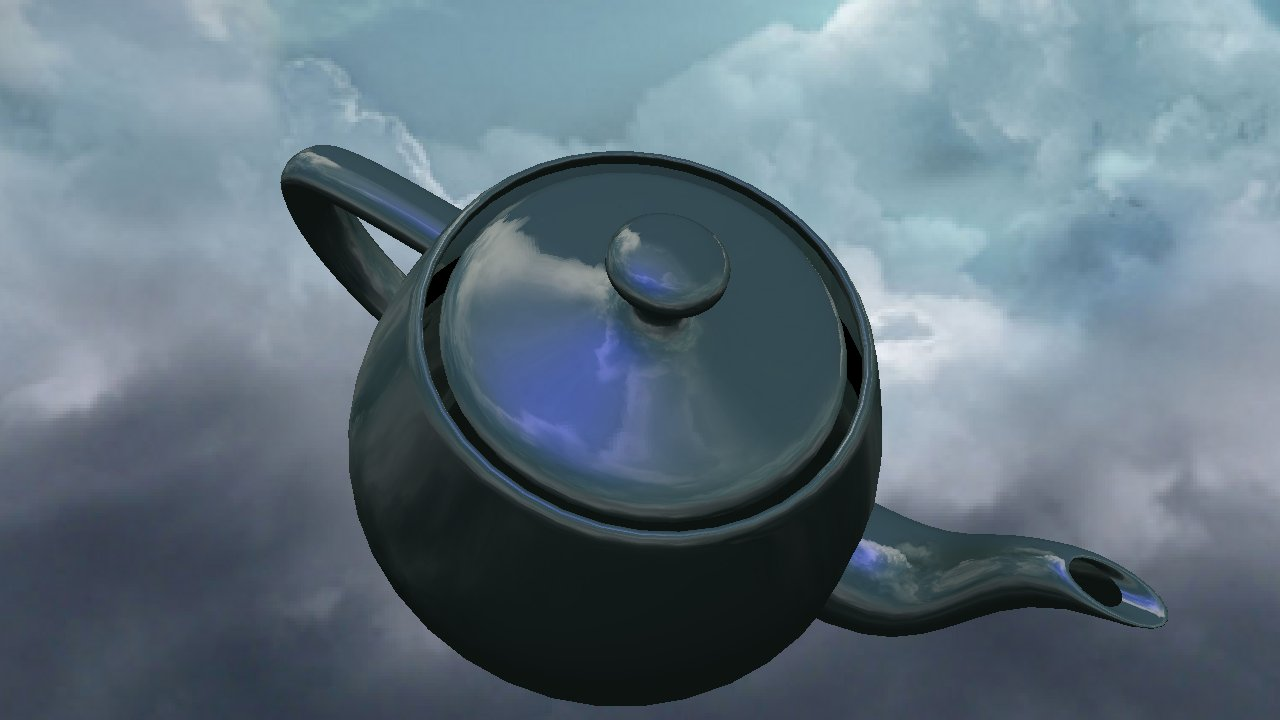
\includegraphics[width=0.9\linewidth]{images/reflection_map.jpg}
\end{figure}

\end{frame}


\section{Screen Space Ambient Occlusion}

\subsection{Principles}

\begin{frame}
\frametitle{Screen Space Ambient Occlusion}
% crytek-crysis 2007
Screen Space Ambient Occlusion (SSAO):
\begin{itemize}
    \item first approach to real time AO
    \item developed at \emph{Crytek GmbH} and included in \emph{CryEngine 2}
    \item used in \emph{Crysis} (2007)
\end{itemize}

\begin{columns}
    \begin{column}{0.4\linewidth}
        \begin{figure}
        \centering
        \subfloat{
\includegraphics[width=0.5\linewidth]{images/crytek_logo.pdf}} \\
        \subfloat{
\includegraphics[width=0.8\linewidth]{images/cryengine_logo.pdf}}
        \end{figure}
    \end{column}

    \begin{column}{0.4\linewidth}
        \begin{figure}
        \centering
        
\includegraphics[width=\linewidth]{images/crysis_cover.png}
        \end{figure}
    \end{column}
\end{columns}

\end{frame}

\begin{frame}
\frametitle{SSAO in Crysis I}
% mettere immagine crysis coreano + tank + muro dietro
\begin{figure}
    \centering
    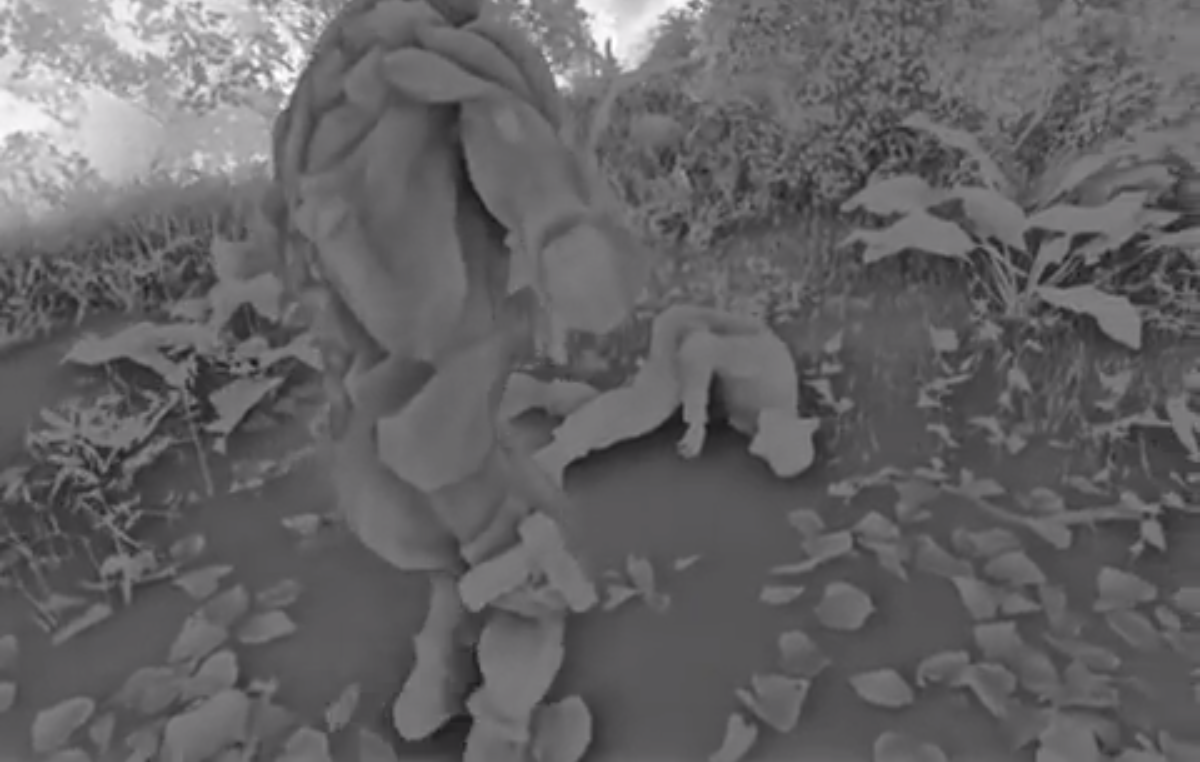
\includegraphics[width=0.8\linewidth]{images/ssao_crysis_gameplay.png}
\end{figure}
\end{frame}

\begin{frame}
\frametitle{SSAO in Crysis II}
\begin{figure}
    \centering
    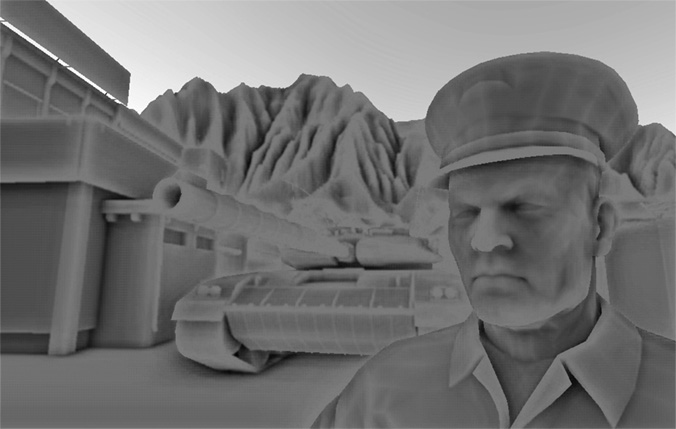
\includegraphics[width=0.8\linewidth]{images/ssao_tank.jpg}
\end{figure}

\end{frame}

\begin{frame}
\frametitle{Screen Space}
SSAO is a \emph{screen space} (ss) technique:
\begin{itemize}
    \item uses \emph{deferred rendering} to split geometry render from light computation:
    \begin{itemize}
        \item pass 1: render geometry/depth in off-screen buffers (g-buffer)
        \item pass 2: use g-buffer's rendered scene as texture to apply lighting
    \end{itemize}
    \item ss effects applied in pass 2 $ \Rightarrow $ screen space resolution dependent
    \item application of ss techniques does not depend on scene complexity (roughly)
\end{itemize}
\end{frame}

\begin{frame}
\frametitle{Deferred Rendering Pipeline}
\begin{figure}
    \centering
    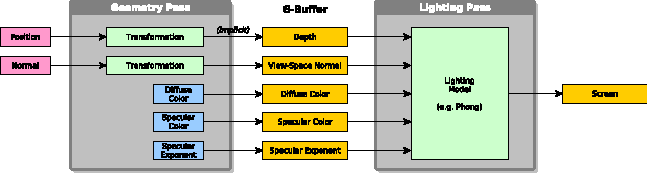
\includegraphics[width=0.9\linewidth]{images/deferred_rendering.pdf}
\end{figure}

\SetKwFor{ForEach}{for each}{}{}
\begin{columns}
    \begin{column}[t]{0.44\linewidth}
        Forward rendering: $\mathcal{O}(N L R)$
        \smaller
        \begin{algorithm}[H]
            \ForEach{object}{
                \ForEach{fragment}{
                    \ForEach{light}{
                        compute lighting\;
                    }
                }
            }
        \end{algorithm}
    \end{column}
    
    \begin{column}[t]{0.44\linewidth}
        Deferred rendering: $\mathcal{O}((N{+}L)R)$
        \smaller
        \begin{algorithm}[H]
            \ForEach{object}{
                \ForEach{fragment}{
                    fill g-buffer\;
                }
            }
            \ForEach{light}{
                \ForEach{fragment}{
                    fetch g-buffer\;
                    compute lighting\;
                }
            }
        \end{algorithm}
    \end{column}
\end{columns}
\end{frame}

\begin{frame}
\frametitle{SSAO Approach}
SSAO fundamental ideas:
\begin{itemize}
    \item leverage deferred rendering (post processing)
    \item use available geometry info to approximate indirect lighting
    \item use of depth buffer for geometry reconstruction (more on this later)
    \item computation of a screen space occlusion map based on geometries surrounding current rasterized fragment
    \item blending of occlusion map with ambient lighting to shade appropriate portions of the image
\end{itemize}
\end{frame}

\begin{frame}
\frametitle{Crytek SSAO}
Crytek's original implementation was never released. High level description available in  \emph{``Finding Next Gen\textemdash{}CryEngine 2''} paper from Crytek.

%Algorithm's high level pseudocode:
%\RestyleAlgo{plain}
\SetKwFor{ForEach}{for each}{}{}
%\SetKwIF\If{cond}{Then’s text}
\SetKwIF{If}{ElseIf}{Else}{if}{}{else if}{else}{endif}
\begin{algorithm}[H]
    render geometry\;
    \ForEach{fragment \textup{in geometry g-buffer}}{
        reconstruct \emph{fragment}'s view space position\;
        sample some points in view space neighborhood\;
        \ForEach{sample}{
            project \emph{sample} in clip space\;
            \If{sample \textup{is behind rasterized geometry}}{
                increment occlusion for current \emph{fragment}\;
            }
        }
        average occlusion for current \emph{fragment} on all \emph{samples}\;
        write $ (1 - \mathit{occlusion}) $ to texture\;
    }
    blend AO map with ambient lighting\;
    \caption{SSAO high level pseudocode.}
\end{algorithm}

\end{frame}

\begin{frame}
\frametitle{SSAO Scheme}
TODO: labels
\begin{figure}
    \centering
    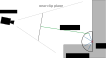
\includegraphics[width=0.9\linewidth]{images/ssao_scheme}
\end{figure}

\end{frame}

\subsection{Implementation Details}
% scrivere che si usa deferred rendering, scrivere tutti i gbuffer che si usano, ..


\begin{frame}[fragile]
\frametitle{Sample kernel}
Uniform variable in fragment shader:
\begin{minted}[bgcolor=bg,fontsize=\footnotesize]{glsl}
uniform vec3 sample_kernel[KERNEL_SIZE];
\end{minted}

Consists in an array of \emph{random} vectors s.t. for each vector $ k $ it holds:
\begin{align*}
-1 & \le k.x \le 1 \\
-1 & \le k.y \le 1 \\
0 & \le k.z \le 1
\end{align*}

Forms a hemisphere centered on the origin $ (0, 0, 0) $ $ \Rightarrow $ Use \emph{tangent space}. Must be reoriented inside the shader.
\end{frame}

\begin{frame}[fragile]
\frametitle{Non-Uniformly Distributed Samples}
Samples near the origin are more interesting: use \emph{accelerating interpolation function} to scale the samples:
\begin{minted}[bgcolor=bg,fontsize=\footnotesize]{c++}
float scale = (float)i / KERNEL_SIZE; // i is the loop variable
scale = lerp(0.1f, 1.0f, scale * scale);
sample *= scale;
\end{minted}

\vspace{0.3cm}

\begin{columns}
    \begin{column}{0.45\linewidth}
        \centering
        Uniform samples:
        \begin{figure}
            \centering
            \vspace{-1.8ex}%
            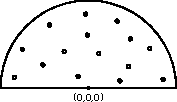
\includegraphics[width=0.7\linewidth]{images/sample_kernel_uniform.pdf}
        \end{figure}
    \end{column}
    
    \begin{column}{0.45\linewidth}
        \centering
        \textbf{Non uniform samples}:
        \begin{figure}
            \centering
            \vspace{-1.8ex}%
            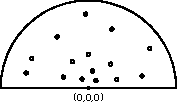
\includegraphics[width=0.7\linewidth]{images/sample_kernel_accel.pdf}
        \end{figure}
        
    \end{column}
\end{columns}

\end{frame}

\begin{frame}[fragile]
\frametitle{Random Kernel Rotations}
To obtain convincing results, a high number of samples must be used $ \Rightarrow $ High memory usage

Solution: use a random $ 4\times4 $ noise texture \emph{tiled} over the screen to rotate the samples.
\begin{minted}[bgcolor=bg, fontsize=\footnotesize]{c++}
noise_texture[i] = Vector3(random(-1,1), random(-1,1), 0);
\end{minted}
\vspace{-1cm}
\begin{minted}[bgcolor=bg, fontsize=\footnotesize]{c++}
glTexParameteri(GL_TEXTURE_2D, GL_TEXTURE_WRAP_S, GL_REPEAT);
glTexParameteri(GL_TEXTURE_2D, GL_TEXTURE_WRAP_T, GL_REPEAT);
\end{minted} 

Random rotation vectors with z-component equal to 0: in tangent space this describes a rotation around z-axis, that is, around the normal.

\end{frame}

\begin{frame}
\frametitle{Samples Reorientation I}
Samples in tangent space must be transformed to view space and shifted by the current fragment's view position.

\emph{Gram-Schmidt process}: orthonormalization of linearly independent vectors to obtain an orthonormal base.

Transformation matrix:
\[
\text{TBN} = 
\begin{bmatrix}
\vec{t} & \vec{b} & \vec{n}
\end{bmatrix} \in \mathbb{R}^{3\times3}
\]
where $ \vec{t} $ is the tangent, $ \vec{b} $ is the bitangent and $ \vec{n} $ is the normal.

Matrix application:
\[ \vec{v}_{\text{view-space}} = \text{TBN} \; \vec{v}_{\text{tangent-space}} \]
\end{frame}

\begin{frame}[fragile]
\frametitle{Sample Reorientation II}

TBN creation in fragment shader:
\begin{minted}[bgcolor=bg, fontsize=\footnotesize]{glsl}
vec3 tangent = normalize(noise - normal * dot(noise, normal));
vec3 bitangent = cross(normal, tangent);
mat3 tbn = mat3(tangent, bitangent, normal);
\end{minted}

\begin{figure}
    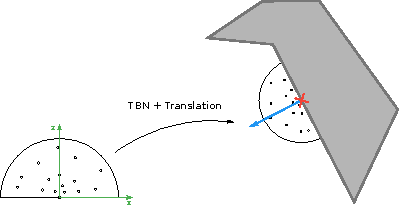
\includegraphics[width=0.7\linewidth]{images/kernel_reorientation.pdf}
    \centering
\end{figure}

\end{frame}

\begin{frame}[fragile]
\frametitle{Sample Reorientation III}
SSAO shader main loop.

To get a sample's view position:
\begin{itemize}
    \item reorient sample
    \item adjust radius
    \item add origin point (fragment's view space)
\end{itemize}
\begin{minted}[bgcolor=bg, fontsize=\footnotesize]{glsl}
float occlusion = 0.0;
for (int i = 0; i < KERNEL_SIZE; ++i) {
    // get sample position:
    vec3 sample_point = tbn * sample_kernel[i];
    sample_point = (sample_point * kernel_radius) + origin;
    ...
\end{minted}

\end{frame}

\begin{frame}
\frametitle{Projection}

\end{frame}

\begin{frame}
\frametitle{Depth Comparison}

\end{frame}

\begin{frame}
\frametitle{Occlusion Computation}

\end{frame}


% Qui metto tutte subsub con le tecniche che ho usato: tipo range check, min/max distance,.. No view space reconstruction. Quella ha subsection dedicata
\subsubsection{Range Check}
\subsubsection{Distance Constraints}

% FIXME: forse usare dei frame più che delle subsubsection per la roba sopra

\subsection{View Space Reconstruction}

\section{Results}

\begin{frame}
\frametitle{App: SSAO layer}
\begin{figure}
    \centering
    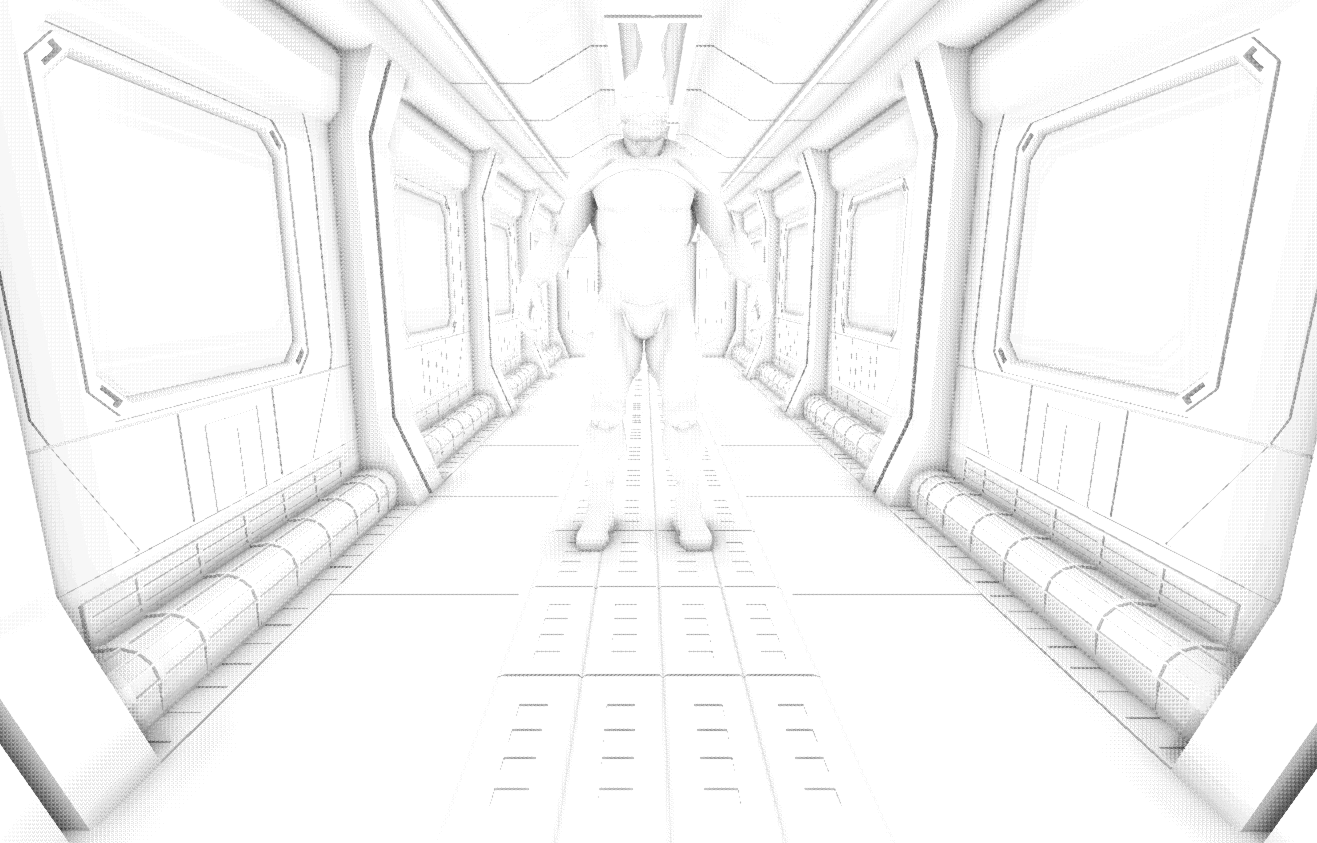
\includegraphics[width=0.95\linewidth]{images/app_ssao}
\end{figure}

\end{frame}



\section{Tools and Software}
% threejs webgl buildpack node/npm heroku eslint

\section{Conclusions}
% future work: depth-aware blur

\section{?Problems? (Insert somewhere)}
% halo effect on object
% problem in calibrating parameters as every other paremetric techinques
% highly dependent on scale of the scene
% corrections help with results but give even more parameters

% ##################### END #####################

\end{document}